\documentclass{article}

% Final report, MIA 5150 (due 4 Dec 2026; 6 pages max, not counting references and the contributions
% appendix). Typeset from ../../final-report-draft.md (2026-11-17); every number is copied from that draft,
% which names its trial record. Red [OWNER: ...] marks are open items for the owner.
% Same style option as the proposal: "preprint" prints the author name.
\usepackage[preprint]{neurips_2026}

\usepackage[utf8]{inputenc}
\usepackage[T1]{fontenc}
\usepackage{hyperref}
\usepackage{url}
\usepackage{booktabs}
\usepackage{tabularx}
\usepackage{amsfonts}
\usepackage{amsmath}
\usepackage{nicefrac}
\usepackage{microtype}
\usepackage{xcolor}
\usepackage{graphicx}
\usepackage{enumitem}
\usepackage{tikz}
\usetikzlibrary{positioning,arrows.meta}
\hypersetup{colorlinks=true,allcolors=blue!50!black}

\newcolumntype{Y}{>{\raggedright\arraybackslash}X}
\newcommand{\owner}[1]{\textcolor{red}{\textbf{[OWNER: #1]}}}
\newcommand{\proposed}{\textcolor{blue}{\textsuperscript{[proposed 2026-11-17]}}}
\newcommand{\code}[1]{\texttt{#1}}
\setlist{nosep,leftmargin=*}

\title{Flags, Not Graphs: What Helps an AI Coding Agent\\with a Self-Contradicting Specification}

\author{%
  Victor Truong \\
  Student number 300264088 \\
  MIA 5150, University of Ottawa \\
  ntruo093@uottawa.ca \\
}

\begin{document}

\maketitle

\begin{abstract}
Spec-driven development (SDD) has an AI coding agent build from a written specification of requirements,
constraints and acceptance criteria rather than from ad-hoc prompts. A main weakness is specification
drift: two documents, or two paragraphs, say different things. In earlier work we built \code{sddc}, a
compiler that turns a folder of Markdown specifications into a graph of quoted requirements and reports
each pair it judges contradictory. This project asks \textbf{whether an agent builds better software from
that graph than from the Markdown}. In controlled runs of Claude Code (Claude Haiku and Sonnet) on six
public Zero2Repo cases (4\,800--19\,000 words, 197--476 hidden tests) with 12--24 planted contradictions,
the graph neither raised nor lowered hidden-test scores. What changed was \textbf{whether the agent noticed
and reported the contradictions}: when they were flagged, the agent named far more of them, in all six
cases and for both models (sign test $p = 0.031$). A plain conflict list from a one-pass LLM review,
given beside the Markdown, did the same, and when a person added a ruling to each listed conflict, the
agent built the ruling almost every time (118 of 120). No format changed how often the agent silently
invented facts removed from the specification. For specifications that fit one agent's context,
\textbf{the useful artefact is a checked list of conflicts with rulings, not a graph}.
\end{abstract}

% ------------------------------------------------------------------ 1
\section{Introduction}

Coding agents now build whole repositories from documents
\citep{chen2026repo0,peng2026repogenesis,yang2026zero2repo}. Spec-driven development makes the documents the source of truth;
but a product requirements document (PRD) and an interface contract written by different people, or
revised at different times, contradict each other, and an agent that does not notice builds one side
silently. Our proposal claimed that \emph{an agent produces code of higher quality from a structured,
graph-based specification than from the same specification as flat files}. We built the graph
(\S\ref{sec:compiler}) and tested the claim under tight controls. The claim as proposed is \textbf{not
supported}, and the experiments say what to do instead. Our contributions:
\begin{enumerate}
  \item A controlled benchmark design for specification conflicts and gaps: contradictions and removed
  facts planted into public Zero2Repo specifications, each chosen so that a black-box probe tells which
  side was built and at most three hidden tests depend on it, with the answer key written before any
  model call (\S\ref{sec:planted}).
  \item Evidence on six cases and two models that a compiled graph does not change hidden-test scores,
  while \textbf{flagged} conflicts are named far more often, and only the flagged ones
  (\S\ref{sec:core}--\ref{sec:naming}).
  \item A baseline the literature and our proposal lacked: the conflict list from a plain LLM review,
  handed to the agent beside the Markdown, carries the same help without the compiler, and with a
  person's rulings added it decides what is built (\S\ref{sec:list}).
  \item A negative result on hallucination: no format makes an agent say that the specification is silent
  (\S\ref{sec:silent}).
\end{enumerate}

% ------------------------------------------------------------------ 2
\section{Related work}

\textbf{Repository-level generation from documents.} SWE-bench \citep{jimenez2024swebench} and SWE-agent
\citep{yang2024sweagent} evaluate edits to existing code; ProjectEval \citep{liu2025projecteval}, DevBench
\citep{kumarappan2026devbench}, RepoGenesis \citep{peng2026repogenesis} and Repo0 \citep{chen2026repo0}
build projects from descriptions. Zero2Repo \citep{yang2026zero2repo} gives a PRD and an interface contract per case and
scores the build with hidden tests; we use it because its tests are written against a stated contract.
None of these plants contradictions in the specification. \textbf{Requirements to code.} TraceDev
\citep{chen2026tracedev} and WiseSpec \citep{tian2026wisespec} use requirements traceability inside
multi-agent pipelines; we instead test whether a compiled specification helps an off-the-shelf agent.
\textbf{Hallucination in code.} Taxonomies \citep{liu2024halucode,zhang2025hallucination,lee2025hallucination}
include code that contradicts or goes beyond the requirements; we measure the second kind as \emph{silent
invention} of facts removed from the specification. \textbf{Context and format.} Long inputs degrade
reasoning \citep{liu2024lost,levy2024moretokens}, and prompt format alone moves scores
\citep{he2024format,sclar2024format}; our export is 3--6$\times$ the Markdown's length, so format effects are a
live confound (\S\ref{sec:limits}). GraphRAG \citep{edge2024graphrag} motivated the graph.
\textbf{Evaluation.} We test each claim over cases (t-test, sign test, non-inferiority and equivalence
bounds) and report counts and ranges, following \citet{miller2024errorbars} on small-$n$ evaluations, and use
an LLM second reader with agreement reported, as LLM-as-judge work advises
\citep{zheng2023judge,crupi2025judge}.

% ------------------------------------------------------------------ 3
\section{Method}

\subsection{Platform}

Claude Code 2.1.316, run headless by Harbor 0.24.0 \citep{harbor_docs} in a Docker container with tools
\code{Bash}, \code{Edit}, \code{Read}, \code{Write}, no dollar ceiling, and a 7\,200\,s agent limit. The agent's
container holds only the specification; hidden tests are copied in after it stops. Coding agents:
\code{claude-haiku-5-5} and \code{claude-sonnet-5-5}. Each condition is one frozen Harbor task, and the arms of
a round differ only in the specification folder and one instruction sentence (\code{diff -r} checked). A
driver runs each round's queue unattended in a fixed interleaved order and reruns, once, a run cut off by
a usage limit or stopped early by an output-limit cut (a rule written before any run). One instruction
line, identical in all arms, asks the agent to list each disagreement it finds in \code{NOTES.md}, stating
both sides, and each point the specification does not state.

\subsection{The compiler and its export}\label{sec:compiler}

\begin{figure}[t]
\centering
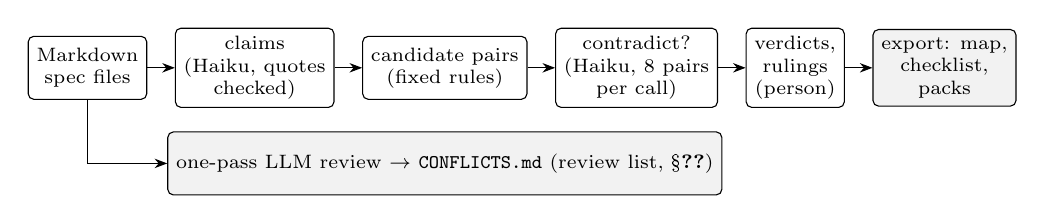
\begin{tikzpicture}[font=\scriptsize, node distance=3.5mm,
  box/.style={draw, rounded corners=2pt, align=center, inner sep=3pt, minimum height=8mm},
  arr/.style={-{Stealth[length=1.6mm]}}]
\node[box] (md) {Markdown\\spec files};
\node[box, right=of md] (cl) {claims\\(Haiku, quotes\\checked)};
\node[box, right=of cl] (pr) {candidate pairs\\(fixed rules)};
\node[box, right=of pr] (ju) {contradict?\\(Haiku, 8 pairs\\per call)};
\node[box, right=of ju] (ve) {verdicts,\\rulings\\(person)};
\node[box, right=of ve, fill=black!5] (ex) {export: map,\\checklist,\\packs};
\draw[arr] (md) -- (cl); \draw[arr] (cl) -- (pr); \draw[arr] (pr) -- (ju);
\draw[arr] (ju) -- (ve); \draw[arr] (ve) -- (ex);
\node[box, below=4mm of pr, fill=black!5] (rv) {one-pass LLM review $\rightarrow$ \code{CONFLICTS.md} (review list, \S\ref{sec:list})};
\draw[arr] (md.south) |- (rv.west);
\end{tikzpicture}
\caption{The compiler \code{sddc} (top) and the plain review list, a second source of flags (bottom).}
\label{fig:pipeline}
\end{figure}

\code{sddc} (Figure~\ref{fig:pipeline}) splits each Markdown file into blocks, asks Claude Haiku which claims
each block makes (every quote is checked word for word against the source), picks candidate pairs by
fixed rules, and asks Haiku, 8 pairs per call, whether two claims duplicate or contradict. A person then
marks false alarms and may record rulings. \code{sddc export} writes a map, a checklist of every claim id and
one \emph{pack} per area: the original text, its claims, and each open conflict with both sides quoted.
The compiler uses Haiku only.

\subsubsection{Why a compiler and not retrieval (RAG)\proposed}\label{sec:rag}

A retrieval-augmented system \citep{lewis2020rag} splits the documents into chunks,
embeds them, and gives the model the $k$ chunks most similar to a query; GraphRAG
\citep{edge2024graphrag} adds an entity graph and community summaries for questions about a whole corpus.
We built a compiler instead, for four reasons recorded in our design notes before any trial; no RAG
baseline was run (\S\ref{sec:limits}).
\textbf{(1) Conflict detection has no query.} Retrieval ranks chunks against a question and returns the
best few. A contradiction check must compare every claim with every other claim on the same subject, and
a pair it never compares fails silently. The compiler extracts every claim and picks candidate pairs by
fixed rules over all claims, so which pairs were compared is set by rules a person can read, and a miss
can be traced to a rule.
\textbf{(2) Similarity is the wrong signal.} Embeddings measure whether two passages read alike; a conflict
is two statements about the same subject that disagree, and they need not read alike. Similarity groups an
\emph{upload size limit} with a \emph{download rate limit}, but separates a \emph{share-link expiry} rule
from the \emph{expiry timestamp} field. Our side B is written in the specification's own voice, often in
another file (30 of 71 planted pairs on four cases); what ties it to side A is its subject, not its
wording.
\textbf{(3) Building code needs the whole specification, with proof of completeness.} An agent must
implement every requirement, not the $k$ most relevant to some question; a chunk left out becomes a missing
feature. The export hands over all the text plus a checklist of every claim id and each open conflict
with both quotes, so what the agent was given can be audited.
\textbf{(4) Rulings need a stable home.} Each claim keeps its quote and id, a person's ruling is attached
to a conflict id and survives a rebuild, and the model only answers narrow, schema-bound questions. A RAG
index stores chunks, not claims or verdicts.
The results narrow this argument: our specifications fit one context, so no selection step was needed at
all, and a plain list from a one-pass review of the whole text helped the agent at least as much as
the compiler's flags (\S\ref{sec:list}). Specifications larger than one context, the target of both retrieval and the
compiler's incremental design, are untested.

\subsection{Planted conflicts and gaps}\label{sec:planted}

No public benchmark ships self-contradicting specifications, so we planted them. For each case an answer
key was written before any compile or run. A \textbf{conflict} keeps the original sentence (side A, what the
hidden tests check) and adds one sentence elsewhere in the specification's own voice that says otherwise
(side B). Each item must (i) be built in earlier unplanted runs, (ii) be readable by a black-box probe on
the saved code, and (iii) change at most three hidden tests between sides, measured with no model by
patching a reference build to each side. A \textbf{gap} removes every statement of a fact the tests still
check, with no marker. The tests touched by any item (the \emph{footprint}) are left out of the
\textbf{core score}, because they reward side A whether or not the agent noticed; the specification does not
say A is right. Table~\ref{tab:cases} lists the cases. Round 28 planted the three new cases with the same
rules; all four arms ran on each, interleaved in one queue.

\begin{table}[t]
\caption{Cases. Words of the planted specification; hidden tests; planted conflicts and gaps; core = tests
outside the footprint.}
\label{tab:cases}
\centering\small
\begin{tabular}{lrrrrrl}
\toprule
Case (upstream library) & Words & Tests & Conflicts & Gaps & Core & Rounds \\
\midrule
case006 (\code{click})    & 14\,435 & 476 & 24 & --- & 445 & 18, 25, 27 \\
case010 (\code{nltk})     &  8\,412 & 197 & 15 & 14 (round 20) & 173 / 175 & 19, 20, 25, 27 \\
case016 (\code{sloptrim}) & 18\,845 & 388 & 17 & 15 & 338 & 21, 23, 24 \\
case005 (\code{h11})      &  7\,916 & 395 & 17 & 11 & 335 & 28 \\
case011 (\code{jmespath}) &  6\,909 & 321 & 12 & 12 & 271 & 28 \\
case001 (\code{tomli})    &  4\,801 & 302 & 15 & 4  & 265 & 28 \\
\bottomrule
\end{tabular}
\end{table}

\subsection{Arms}

\textbf{Markdown:} the planted specification as given. \textbf{Compiler export:} \code{sddc export} of the
planted specification, false contradictions removed by verdicts, nothing added. \textbf{Oracle export:} the
compiler export plus the planted conflicts it missed, injected from the answer key: an upper bound for a
perfect compiler. \textbf{Review list:} the Markdown plus \code{CONFLICTS.md} from one plain LLM review of the
same Markdown (asked only to list contradictions, no code), unfiltered, chosen by a fixed rule (the first Haiku review of the case).
\textbf{Settled list} (case016 only): the review list with its false entries struck and a ruling added to
each entry; the planted side B is ruled on alternate entries so that following the ruling can be told from
default behaviour.

\subsection{Measures and readers}

\textbf{Set 1, core:} hidden tests passed outside the footprint. \textbf{Set 2a, named:} under a strict rule
fixed before the runs, \code{NOTES.md} states the content of both sides and presents them as a choice; an id
or topic alone does not count. \textbf{Set 2b, silent inventions:} gaps whose value the code takes while the
notes do not name it as unstated. \textbf{Built side:} the probe's reading. Cost is Claude Code's
\code{total\_cost\_usd}, an API-price estimate (the runs used a subscription). Reader 1 (the assistant in
Claude Code) read every \code{NOTES.md} item by item, not blind to arm. \textbf{Reader 2} (Claude Sonnet, no
tools, a fresh context per run) read the same files under the same rule, blind to run, arm, model and
reader 1, and we report Cohen's $\kappa$.

\subsection{Sample size and tests}\label{sec:stats}

The claims are about specifications in general, so the \textbf{unit of analysis is the case}; runs inside a
case only make that case's mean more precise. Each model is analysed on its own. For each case we take
the arm's mean minus the Markdown's mean, then test the $K$ case differences.
\textbf{Naming (superiority):} two-sided one-sample t-test, $\alpha = 0.05$, and a sign test, which needs all
cases in one direction and $K \ge 6$ (two-sided $p = 2 \cdot 0.5^K = 0.031$). \textbf{Core
(non-inferiority):} the one-sided 95\,\% lower bound of the mean difference lies above $-\delta$, with
$\delta = 2$ points for Sonnet and 5 for Haiku (about $1.5\times$ each model's run-to-run spread, fixed before
rounds 21--25). \textbf{Silent invention (equivalence):} the 90\,\% interval lies inside $\pm 2$ gaps per run.
A power simulation on the first three cases (4\,000 studies per cell) showed that more cases raise power
far more than more runs per case; we therefore set \textbf{6 cases with planted conflicts, at least 4 with
planted gaps, and 5 Haiku and 3 Sonnet runs per arm per case}, and ran the extra cases as round 28.
Table~\ref{tab:tests} gives the tests on all six cases.

\begin{table}[t]
\caption{The claims tested over the six cases: case differences (arm $-$ Markdown, points of \%) in the
order case006, case010, case016, case005, case011, case001. Haiku $n = 5$ runs per cell except $n = 3$ on
case006 and case010; Sonnet $n = 3$.}
\label{tab:tests}
\centering\scriptsize
\setlength{\tabcolsep}{3pt}
\resizebox{\linewidth}{!}{%
\begin{tabular}{lllll}
\toprule
Claim & Model & Six case differences & Test over cases & Status \\
\midrule
Oracle export raises naming & Haiku & $+63.9,+44.4,+29.4,+12.9,+18.3,+33.3$ & t $p=0.007$; sign $p=0.031$ & \textbf{holds} \\
 & Sonnet & $+26.4,+26.7,+15.7,+17.6,+47.2,+51.1$ & t $p=0.004$; sign $p=0.031$ & \textbf{holds} \\
Review list raises naming & Haiku & $+58.3,+35.6,+24.7,+5.9,+16.7,+28.0$ & t $p=0.012$; sign $p=0.031$ & \textbf{holds} \\
 & Sonnet & $+16.7,+20.0,+25.5,+9.8,+38.9,+33.3$ & t $p=0.003$; sign $p=0.031$ & \textbf{holds} \\
Compiler export raises naming & Haiku & $+52.8,+31.1,+14.1,-1.2,+6.7,+26.7$ & t $p=0.041$; 5 of 6 positive & t only \\
 & Sonnet & $+23.6,+17.8,+9.8,-3.9,+30.6,+20.0$ & t $p=0.021$; 5 of 6 positive & t only \\
\midrule
Oracle export, no harm to core & Haiku ($\delta$ 5) & $+4.2,+2.1,+4.1,0.0,0.0,-0.1$ & lower bound $+0.03$ & \textbf{non-inferior} \\
 & Sonnet ($\delta$ 2) & $-0.2,-0.2,-0.4,0.0,+7.1,0.0$ & lower bound $-1.40$ & \textbf{non-inferior} \\
Review list, no harm to core & Haiku ($\delta$ 5) & $+3.6,+2.7,+4.4,-0.4,-4.1,0.0$ & lower bound $-1.59$ & \textbf{non-inferior} \\
 & Sonnet ($\delta$ 2) & $0.0,-0.8,+0.3,0.0,+6.6,0.0$ & lower bound $-1.25$ & \textbf{non-inferior} \\
Compiler export, no harm to core & Haiku ($\delta$ 5) & $+9.7,+2.5,+5.0,0.0,+0.3,0.0$ & lower bound $-0.25$ & \textbf{non-inferior} \\
 & Sonnet ($\delta$ 2) & $-0.4,+0.4,+0.3,0.0,+7.1,-0.5$ & lower bound $-1.27$ & \textbf{non-inferior} \\
\midrule
No format changes silent invention & both ($\delta$ 2 gaps) & 5 cases with gaps (all but case006) & 90\,\% CI inside $\pm 2$, all 6 rows ($K$ 4--5) & \textbf{equivalent} \\
\bottomrule
\end{tabular}}
\end{table}

The silent-invention intervals (arm $-$ Markdown, gaps per run) are, for Haiku, compiler $+0.47$
$[-0.52, +1.46]$, oracle $+0.80$ $[+0.03, +1.57]$, review $+0.15$ $[-0.30, +0.60]$; for Sonnet, $+0.33$
$[-0.17, +0.84]$, $+0.17$ $[-0.51, +0.85]$, $-0.58$ $[-1.45, +0.29]$. Without case001 (only 4 gaps), two rows no
longer fit inside $\pm 2$ at $K = 3$. Measured on all six cases, the run-to-run SD within a cell is 2.53
(Sonnet) and 3.02 (Haiku) core points, 12.1 and 6.7 naming points, and 0.97 gaps. Sonnet's spreads grew from
the plan's because of single runs (\S\ref{sec:core}); re-estimated with them, power at $K = 6$ is 0.97--0.99
for Haiku's core bound and 0.76--0.87 for naming, but 0.59 for Sonnet's 2-point core bound, which all three
Sonnet arms still pass.

% ------------------------------------------------------------------ 4
\section{Results}

\subsection{Code quality does not move}\label{sec:core}

\begin{table}[t]
\caption{Set 1 (core) and set 2a (named): core \% passed (run range) and conflicts named, \% of items
$\times$ runs. Haiku $n = 5$ per cell except $n = 3$ on case006 and case010; Sonnet $n = 3$. case016's core
is in tests of 338.}
\label{tab:main}
\centering\scriptsize
\setlength{\tabcolsep}{2.5pt}
\resizebox{\linewidth}{!}{%
\begin{tabular}{ll*{4}{rr}}
\toprule
 & & \multicolumn{2}{c}{Markdown} & \multicolumn{2}{c}{Compiler export} & \multicolumn{2}{c}{Oracle export} & \multicolumn{2}{c}{Review list} \\
\cmidrule(lr){3-4}\cmidrule(lr){5-6}\cmidrule(lr){7-8}\cmidrule(lr){9-10}
Case (conflicts) & Model & core & named & core & named & core & named & core & named \\
\midrule
case006 (24) & Haiku  & 87.6 (86.1--90.1) & 36.1 & 97.3 (96.2--98.0) & 88.9 & 91.8 (84.5--96.9) & 100 & 91.2 (86.1--96.4) & 94.4 \\
             & Sonnet & 98.6 (98.4--98.7) & 73.6 & 98.2 (98.0--98.4) & 97.2 & 98.4 (98.2--98.7) & 100 & 98.6 (98.4--98.7) & 90.3 \\
case010 (15) & Haiku  & 89.8 (87.3--94.8) & 51.1 & 92.3 (89.0--94.2) & 82.2 & 91.9 (90.8--93.6) & 95.6 & 92.5 (90.2--93.6) & 86.7 \\
             & Sonnet & 97.1 (95.4--98.8) & 66.7 & 97.5 (96.0--98.8) & 84.4 & 96.9 (94.8--98.8) & 93.3 & 96.3 (95.4--98.3) & 86.7 \\
case016 (17) & Haiku  & 312.8 & 64.7 & 329.8 & 78.8 & 326.8 & 94.1 & 327.6 & 89.4 \\
             & Sonnet & 333.0 & 70.6 & 334.0 & 80.4 & 331.7 & 86.3 & 334.0 & 96.1 \\
case005 (17) & Haiku  & 100 & 87.1 & 100 & 85.9 & 100 & 100 & 99.6 (97.9--100) & 92.9 \\
             & Sonnet & 100 & 82.4 & 100 & 78.4 & 100 & 100 & 100 & 92.2 \\
case011 (12) & Haiku  & 99.7 (98.5--100) & 75.0 & 100 & 81.7 & 99.7 (98.5--100) & 93.3 & 95.6 (79.3--100) & 91.7 \\
             & Sonnet & 92.9 (79.3--100) & 52.8 & 100 & 83.3 & 100 & 100 & 99.5 (99.3--100) & 91.7 \\
case001 (15) & Haiku  & 100 & 66.7 & 100 & 93.3 & 99.9 (99.6--100) & 100 & 100 & 94.7 \\
             & Sonnet & 100 & 42.2 & 99.5 (98.5--100) & 62.2 & 100 & 93.3 & 100 & 75.6 \\
\bottomrule
\end{tabular}}
\end{table}

All three export and list arms pass the non-inferiority bound for both models (Table~\ref{tab:tests}). On
the three new cases the core was at or near the ceiling in every arm: 85 of 96 runs passed every core
test. The two low cells come from two runs, a case011 Markdown run (Sonnet) and a case011 review-list run
(Haiku), each at 215 of 271. Both failed the same 56 tests because they gave the error for an unfinished
expression (\code{foo.}) a different kind from the one the tests expect, one of the disagreements already
present in Zero2Repo's own text, so it is not an arm
effect. On the first three cases Haiku's core was higher with every flag source (oracle $+4.2$, $+2.1$,
$+4.1$; review list $+3.6$, $+2.7$, $+4.4$; compiler export $+9.7$, $+2.5$, $+5.0$ points). That pattern did not
repeat on the new cases ($-4.1$ to $+0.3$), and over six cases no arm's gain is significant
($p = 0.10$--$0.47$). Two extra Haiku runs per arm on case006 and case010 (round 27b), made two weeks after
round 18, scored the case006 Markdown higher (97.5 and 91.2\,\% against 86.1--90.1\,\%); with $n = 5$ that
cell's mean rises from 87.6 to 90.3\,\% and the compiler export's gain there falls from $+9.7$ to $+6.2$. We read
the old case006 gap as time or chance. The rules the tests check are stated in both formats; the failures
we read are unspecified algorithms, single edge rules missed in both formats, and coding slips.

\subsection{Flags drive naming, item by item}\label{sec:naming}

With every conflict flagged, both models named 86--100\,\% against 36--87\,\% from the Markdown, a gain in all
twelve case $\times$ model cells (Table~\ref{tab:main}); the new cases start higher from the Markdown, so the
gain there is smaller. The compiler export shows where the gain comes from. It flags 15 of 24, 9 of 15, 10
of 17, 8 of 17, 7 of 12 and 12 of 15 planted conflicts. On the flagged ones, Haiku's naming went from
29--95\,\% in the Markdown to 96--100\,\% in every case, and Sonnet's from 42--96\,\% to 87--100\,\% in five cases
(72\,\% on case001, where one run named 2 of 15). On the unflagged ones, whose both sides sit in the same
packs, the change was small and mixed: $-22$ to $+22$ points over the twelve cells. So the compiler export sits
between the Markdown and the oracle export in ten of twelve cells; the exceptions are case005, where it
flags fewer than half the conflicts (85.9 against 87.1\,\%, 78.4 against 82.4\,\%). A flag with a wrong
rationale did not help: case010's C18, flagged by the compiler as a different clash, was named in 0 of 3
Sonnet runs. The review list repeats this: on the new cases its runs named 311 of 320 listed-conflict
readings, while the unlisted ones gained nothing over the Markdown (8 of 32 readings against 8 of 32).
Naming also changed what was built unnoticed: across rounds 18, 19, 21, 27 and 28 no flagged conflict was
ever built on side B without being named, while Markdown runs did so 35 times. With round 27b ($n = 5$ for
Haiku on case006 and case010) every naming test still passes ($p = 0.004$, $0.007$, $0.033$), although the two
extra case006 Markdown runs named 70.8 and 54.2\,\% against 29--42\,\% in round 18.

\subsection{A review list as the source of flags, and a settled list carries rulings}\label{sec:list}

On case016, the Markdown plus one review list (15 of 17 flagged, 3 false entries) gave 89.4\,\% (Haiku) and
96.1\,\% (Sonnet) naming, against 78.8 and 80.4\,\% from the compiler export, with the same core and the fewest
planted sides built of any arm (1 of 85, 1 of 51). The list's errors travel: its false entry made 5 of 8
runs build a behaviour the PRD rules out, against 0 of 24 runs without the list. On case006 and case010,
207 of 210 listed-conflict readings were named, and the lists' 4 false entries misled no run. On the
three new cases the review list again named more than the compiler export in all six cells, with core
unchanged. \textbf{Settled list} (case016): with the 3 false entries struck and a ruling on each entry (side B
ruled on 7 of 15), agents built 118 of 120 rulings, including 54 of 56 side-B rulings that unruled agents
built 0--2 times per arm; the misleading build disappeared (0 of 8).

\subsection{No format reduces silent invention}\label{sec:silent}

\begin{table}[t]
\caption{Set 2b: silent inventions per run (lower is better), mean over runs. No arm flags any gap.
case010's export is the plain compiler export (round 20).}
\label{tab:silent}
\centering\small
\begin{tabular}{llrrrrr}
\toprule
Case (gaps) & Model & Markdown & Compiler export & Oracle export & Review list & Settled list \\
\midrule
case010 (14) & Haiku  & 10.67 & 11.00 & --- & --- & --- \\
             & Sonnet & 13.33 & 13.33 & --- & --- & --- \\
case016 (15) & Haiku  & 12.4 & 12.4 & 13.2 & 12.8 & 12.8 \\
             & Sonnet & 13.67 & 14.0 & 13.33 & 13.3 & 12.3 \\
case005 (11) & Haiku  & 9.2 & 8.4 & 9.2 & 8.8 & --- \\
             & Sonnet & 9.33 & 10.33 & 10.33 & 9.33 & --- \\
case011 (12) & Haiku  & 4.8 & 6.8 & 6.4 & 5.2 & --- \\
             & Sonnet & 10.0 & 10.67 & 10.0 & 8.33 & --- \\
case001 (4)  & Haiku  & 1.0 & 1.8 & 1.8 & 1.2 & --- \\
             & Sonnet & 3.0 & 2.67 & 3.0 & 2.67 & --- \\
\bottomrule
\end{tabular}
\end{table}

Every arm is equivalent to the Markdown within $\pm 2$ gaps per run (Table~\ref{tab:tests}). Agents filled
most gaps without saying so in every arm and case (Table~\ref{tab:silent}); Sonnet flagged 4 of 84 gap
readings on case010. The exception is Haiku on case011, which named 5--9 of 12 gaps as unstated in each run
(Sonnet 1--4), in every arm: a model difference within one case. The gaps that were flagged were mostly
those a neighbouring sentence still exposed. On \code{nltk} every gap was filled with the real library's
value (168 of 168), so the hidden tests reward the invention; on \code{sloptrim}, which is not on PyPI, five
gaps were filled in every run with a value the tests reject.

% ------------------------------------------------------------------ 5
\section{Analysis}

\textbf{Why tests do not move but naming does.} Every run read both sides of every planted item; the
difference is connecting them. A flag puts both quotes under one heading, which removes the search step;
the agent then names the conflict but mostly builds the original side, so the tests, which check side A,
see little change. \textbf{What carried the gain was the flag, not the graph.} Unflagged conflicts in the
compiler export gained nothing consistent over the Markdown although they sat in the same packs, flagged
ones rose to 87--100\,\% in eleven of twelve cells, and a flat list from a review gave the same gain.
\textbf{Where the compiler still has a place.} Its rulings and checklist are structure a person can
audit. \textbf{Cost.} An export run costs
Haiku 1.6--3.1$\times$ a Markdown run, plus a compile of \$1.45--3.58 est.\ and a verdict on each false
contradiction (203 of the 282 raised). \textbf{What the settled list adds}
is control: a person's rulings, not the agent's default, decide what is built, and striking a false entry
removes the build it caused. \textbf{The measure holds:} an arm-blind second reader read all 3\,336 item
readings; of 21 disagreements, reader 2 was right in 3 (reader 1 corrected) and reader 1 held in 18. After
the corrections the readers agree on 99.5\,\% ($\kappa = 0.980$), and no arm comparison changes.

% ------------------------------------------------------------------ 6
\section{Limitations}\label{sec:limits}

(1) \textbf{One model family and one agent} (Claude in Claude Code). (2) \textbf{Small $n$:} 3--5 runs per
cell, so every claim rests on the test over cases. (3) \textbf{Six cases}, five ported from well-known
libraries the models may remember; on the three new cases the core was at the ceiling, so set 1 there can
show harm but hardly help. (4) \textbf{The planted items were designed by the same assistant that built the
compiler and reads the notes}, with the answer key written before any run. (5) \textbf{Reading
\code{NOTES.md} is a judgement:} reader 1 was not blind to arm; reader 2 is blind by label, not by content,
and from the same model family. Round 24's rulings followed a fixed alternation, not a person's
judgement. (6) \textbf{The export changes more than structure:} it is 3--6$\times$ longer and its map states how
many conflicts are open. (7) \textbf{Specifications fit one context}, so the large-specification case is not
tested. (8) \textbf{Costs are API-price estimates}, not money billed. (9) \textbf{Time:} on case006 and
case010 the arms come from rounds weeks apart, and round 27b shows drift in the Markdown baseline; round 28
interleaved all arms. (10) \textbf{No retrieval (RAG) baseline was run}; \S\ref{sec:rag} argues from the
design. (11) \textbf{The compiler's accuracy as a detector is out of scope}: we measure what its output
does to the agent, so the compiler-export arm is bounded by what the compiler flags.

% ------------------------------------------------------------------ 7
\section{What we learned: a retrospective\proposed}\label{sec:retro}

This is a course project, so we report the process too.
\textbf{(1) A test must be able to fail.} Our first pilot gave the Markdown and the export the same score
(26 of 26 hidden tests): a clean specification leaves nothing for a format to fix. Planting conflicts and
gaps, and leaving their tests out of the core, made formats distinguishable; even so, the core hit its
ceiling on the new cases, so the ceiling needs checking in every case.
\textbf{(2) Build the plainest baseline first.} We compared formats for 21 rounds before asking a model,
with no tools, to list the contradictions; its list gave the agent the same help as the flags, and run
first it would have set the research question weeks earlier.
\textbf{(3) Change one thing at a time, and run arms side by side.} Early rounds changed three conditions
at once, and arms run weeks apart drifted (round 27b); round 28 interleaved all arms.
\textbf{(4) Fix the answer and the reading rule before the runs,} and have a blind second reader check
every reading; it corrected three of ours.
\textbf{(5) Read the logs before calling something a model result.} Early Haiku stops came from an
output-limit cut and a misread budget reminder (13 of 31 Haiku runs in rounds 14--17 hit the cut, 4
misread the budget), not from the model's ability; harness faults had to be told apart from results too.
\textbf{(6) Size the study on the unit of the claim:} cases, not runs.
\textbf{(7) Test the expectation, and keep the negative result.} We expected the graph to help and the
agents to miss what the compiler missed; the data showed neither, and asking why led to the real finding.
\textbf{(8) Working with an AI assistant.} Claude Code wrote most of the code, planted the items and read the
notes, which made 28 rounds possible; the safeguards against one assistant designing and reading were the
answer key written first, black-box probes, fixed rules, the blind second reader, and the owner reviewing
every decision and commit.

% ------------------------------------------------------------------ 8
\section{Conclusion}

A compiled specification graph did not make an AI coding agent's code better on six public cases with
planted contradictions. What helped was telling the agent where the contradictions are: flagged
conflicts were named, and built knowingly, while unflagged ones were not. A plain conflict list from a
one-pass LLM review carried the same help to the agent without the compiler. The
list's errors travel too, so the practical pipeline is: review, let a person strike false entries and
rule, and hand the agent the short settled list beside the specification. Agents still fill silent gaps
without saying so, whatever the format.

\bibliographystyle{plainnat}
\bibliography{references}

\appendix

\section{Contributions}
Victor Truong did all the work: design, implementation, experiments and writing, with the AI assistance
described in Appendix~B.

\section{Use of AI tools}
We used \textbf{Claude Code} (Anthropic) to write the compiler (\code{sddc}) and its tests from our
specifications, the Harbor task builders, the run driver and the scorers; to design and plant the
conflicts and gaps and build the oracle exports; to run and monitor the trials; to read the agents'
\code{NOTES.md} into detection tables (reader 1); to debug runs; and to draft the trial records and this
report. A second Claude model (Sonnet) is reader 2. We used \textbf{GitHub Copilot CLI} to operate one round's
run queue from a written procedure. Claude models are also part of the method: Claude Haiku splits and
compares requirements inside the compiler, and Claude Haiku and Sonnet are the coding agents and reviewers
under test. \owner{state what you checked yourself (figures, citations, code) before submission.}

\section{Reproduction}
Code: the \code{sdd-compiler} repository, \url{https://github.com/VictorTruong89/sdd-compiler}. Every table is produced by a script that reads the
saved runs and needs no model call: per-round \code{notes/tables.py} under \code{harness/trials/}, the review
scorers of rounds 22 and 28, \code{harness/trials/stats/power\_plan.py} (\code{TOPUP=1} adds round 27b), and
\code{r26-second-reader-detection/notes/reader2.py table}. Model runs are not seeded (Claude Code exposes no
seed); the second reader's run codes use \code{random.Random(2611 + n)}.

\end{document}
